% !TeX root = ../thuthesis-example.tex

\chapter{系统分析与设计}

\section{系统用例分析}

在软件工程的需求分析阶段，明确系统边界与用户角色是至关重要的一步。本系统的主要参与者被明确划分为两类：后台运营管理员与前端微信小程序用户。通过对核心业务的梳理，本人构建了系统的顶层用例模型，旨在消除功能边界上的歧义。

\begin{figure}[htbp]
  \centering
  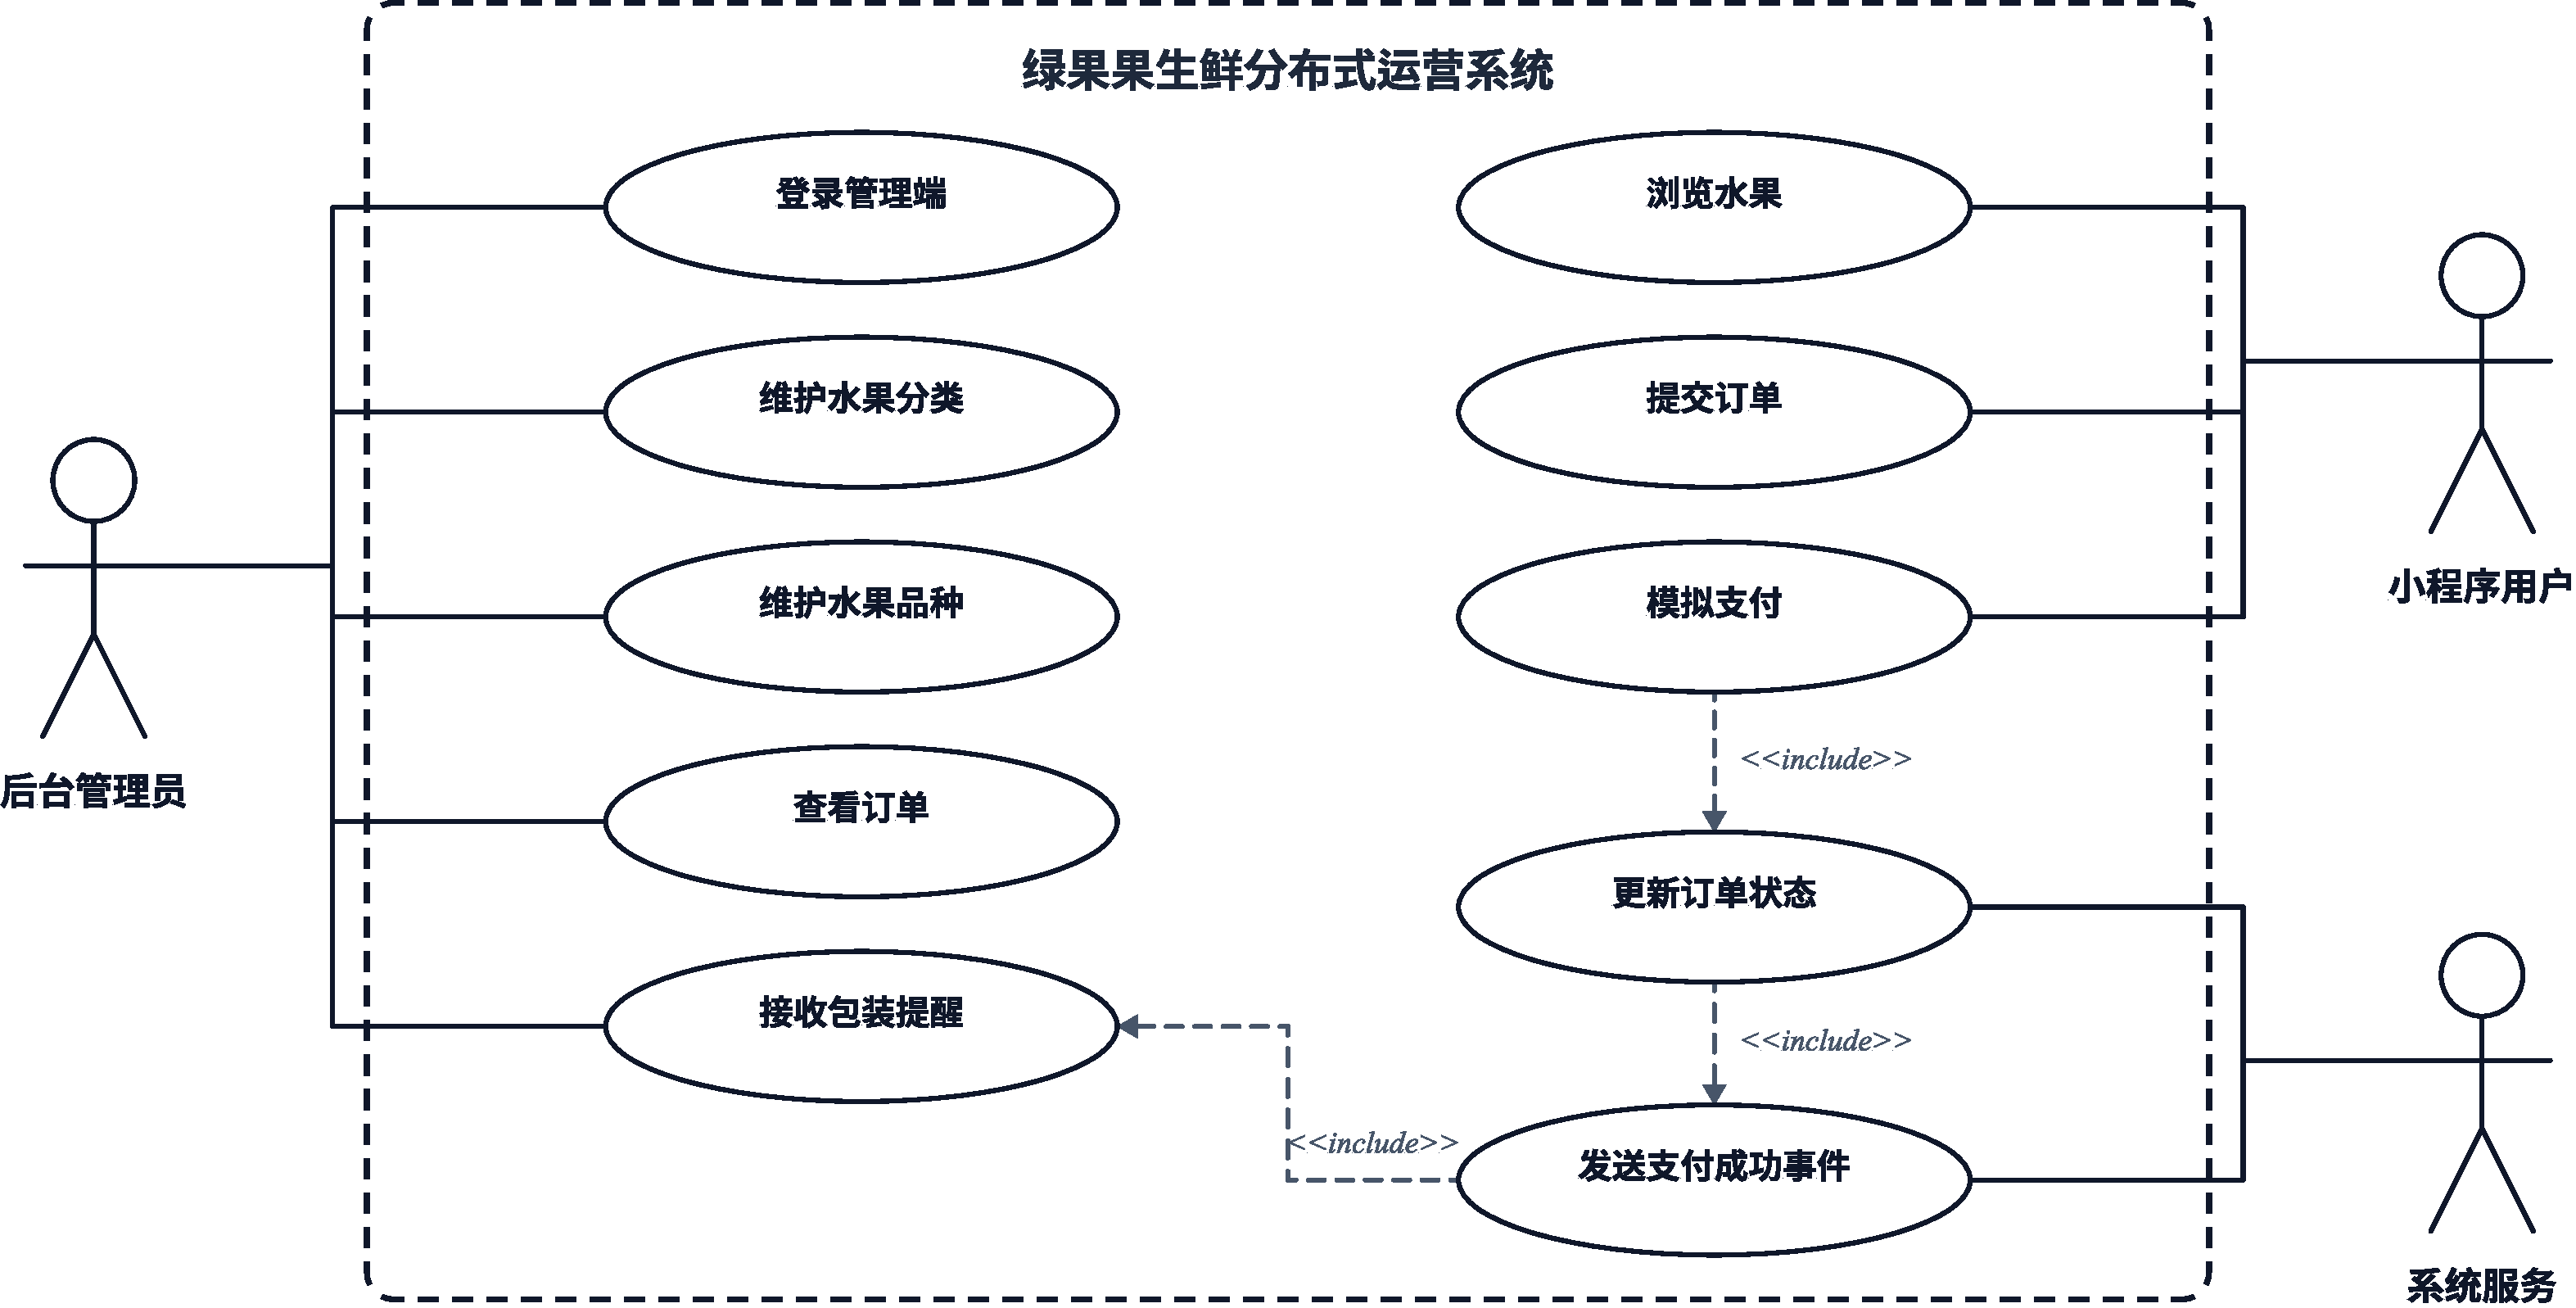
\includegraphics[width=0.9\textwidth]{figures-pdf/用例图.pdf}
  \caption{系统核心用例图}
  \label{fig:U05}
\end{figure}

如图 \ref{fig:U05} 所示，对于后台运营管理员而言，系统提供了基于角色的访问控制（RBAC）。普通运营员被授予水果分类管理、商品品种上下架管理以及订单处理的核心操作权限。超级管理员则额外拥有全系统的最高权限，能够执行用户管理、菜单与角色分配等高危系统配置。这种粒度细分的用例划分，确保了后台管理的职责隔离与最小授权原则。

对于微信小程序用户而言，其用例主要围绕购物闭环展开。用户可以浏览水果分类与商品列表，通过关键字模糊检索特定水果，并将其加入购物车。在确认收货地址后，用户提交订单并发起微信模拟支付，最终在个人中心查看历史订单状态。这些用例完整覆盖了生鲜电商的核心消费旅程。

\section{数据模型与E-R图设计}

在明确了系统的顶层用例后，下一步是基于用例抽取出底层的核心数据字典与实体关系（Entity-Relationship）。系统的核心实体包括水果分类、水果商品、订单以及订单明细。

\begin{figure}[htbp]
  \centering
  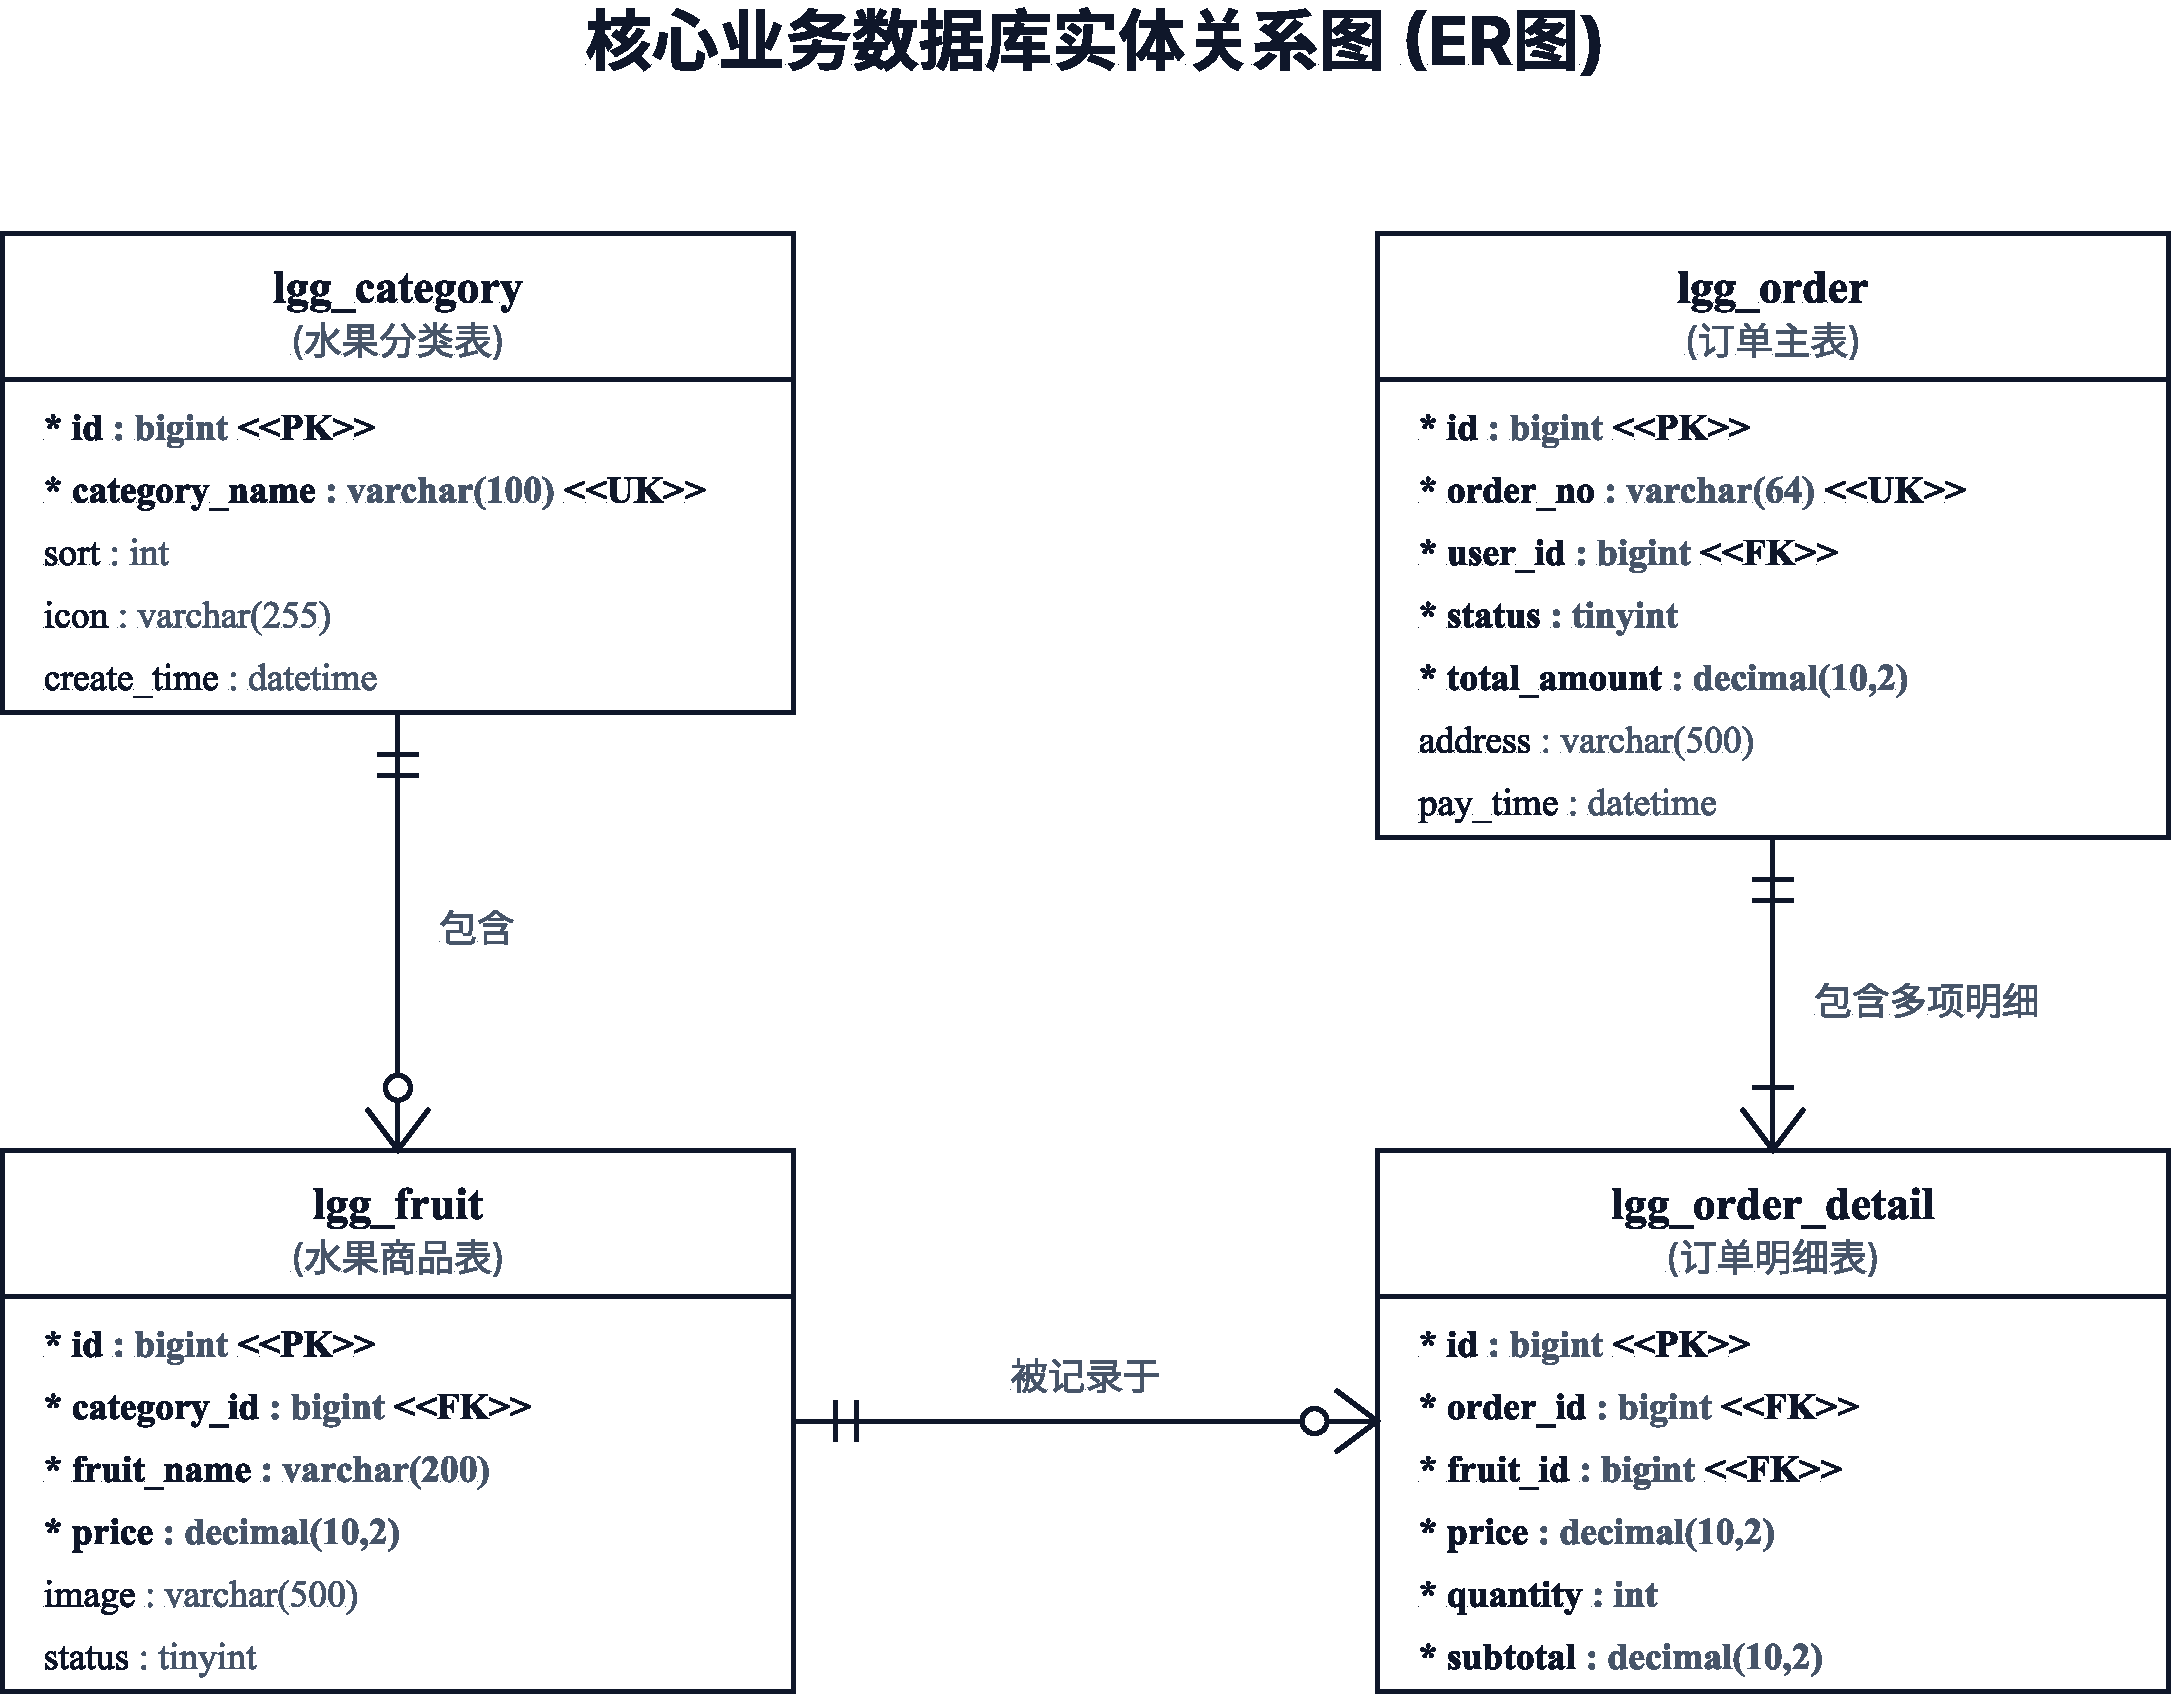
\includegraphics[width=0.9\textwidth]{figures-pdf/U07-database-er.pdf}
  \caption{核心业务数据库实体关系图}
  \label{fig:U07}
\end{figure}

从图 \ref{fig:U07} 可以看出，水果分类（Category）与水果商品（Fruit）之间存在一对多的关联关系。用户与订单（Order）之间同样是一对多的关联，而订单与商品之间则通过订单明细表（Order Detail）构建了多对多的映射。在物理设计上，为了兼顾课程设计展示的低风险性与微服务演进需求，所有业务数据表暂时与若依系统表共存于同一个 MySQL 实例中，但通过逻辑前缀严格隔离。

\begin{table}[htbp]
  \centering
  \caption{核心数据库表与索引设计表}
  \label{tab:database_tables}
  \begin{tabular}{llp{0.35\textwidth}l}
    \toprule
    表名 & 功能说明 & 核心索引列 & 索引类型 \\
    \midrule
    lgg\_category & 存储水果分类信息 & category\_name & 唯一索引 \\
    lgg\_fruit & 存储水果单品与图片 & fruit\_name & 全文索引 \\
    lgg\_order & 存储用户支付订单流转 & order\_no & 唯一索引 \\
    lgg\_order\_detail & 订单下挂载的水果明细 & order\_id & 普通索引 \\
    \bottomrule
  \end{tabular}
\end{table}

表 \ref{tab:database_tables} 展示了核心业务表及其索引策略。本人在分类名和订单号上建立唯一索引以保证数据一致性，在商品名上建立全文索引以支持高效模糊检索。此外，系统在物理层面去除了所有跨表外键约束，转而在应用层代码中保证引用完整性，从而降低了高并发写入时的数据库锁竞争。

\section{技术选型与系统架构设计}

有了稳固的数据模型作为基座，系统进入技术架构选型与宏观架构设计阶段。项目采用当前主流的前后端分离与微服务分布式架构。技术栈方面，后端依托 Spring Boot 3.2.5 框架，利用 Spring Cloud 的 Gateway 网关、OpenFeign 远程调用组件，结合 Nacos 实现服务注册与动态发现；缓存层引入 Redis，对象存储采用 MinIO，消息解耦采用 RabbitMQ。前端则采用 Vue3 与微信小程序原生框架构建。

\begin{figure}[htbp]
  \centering
  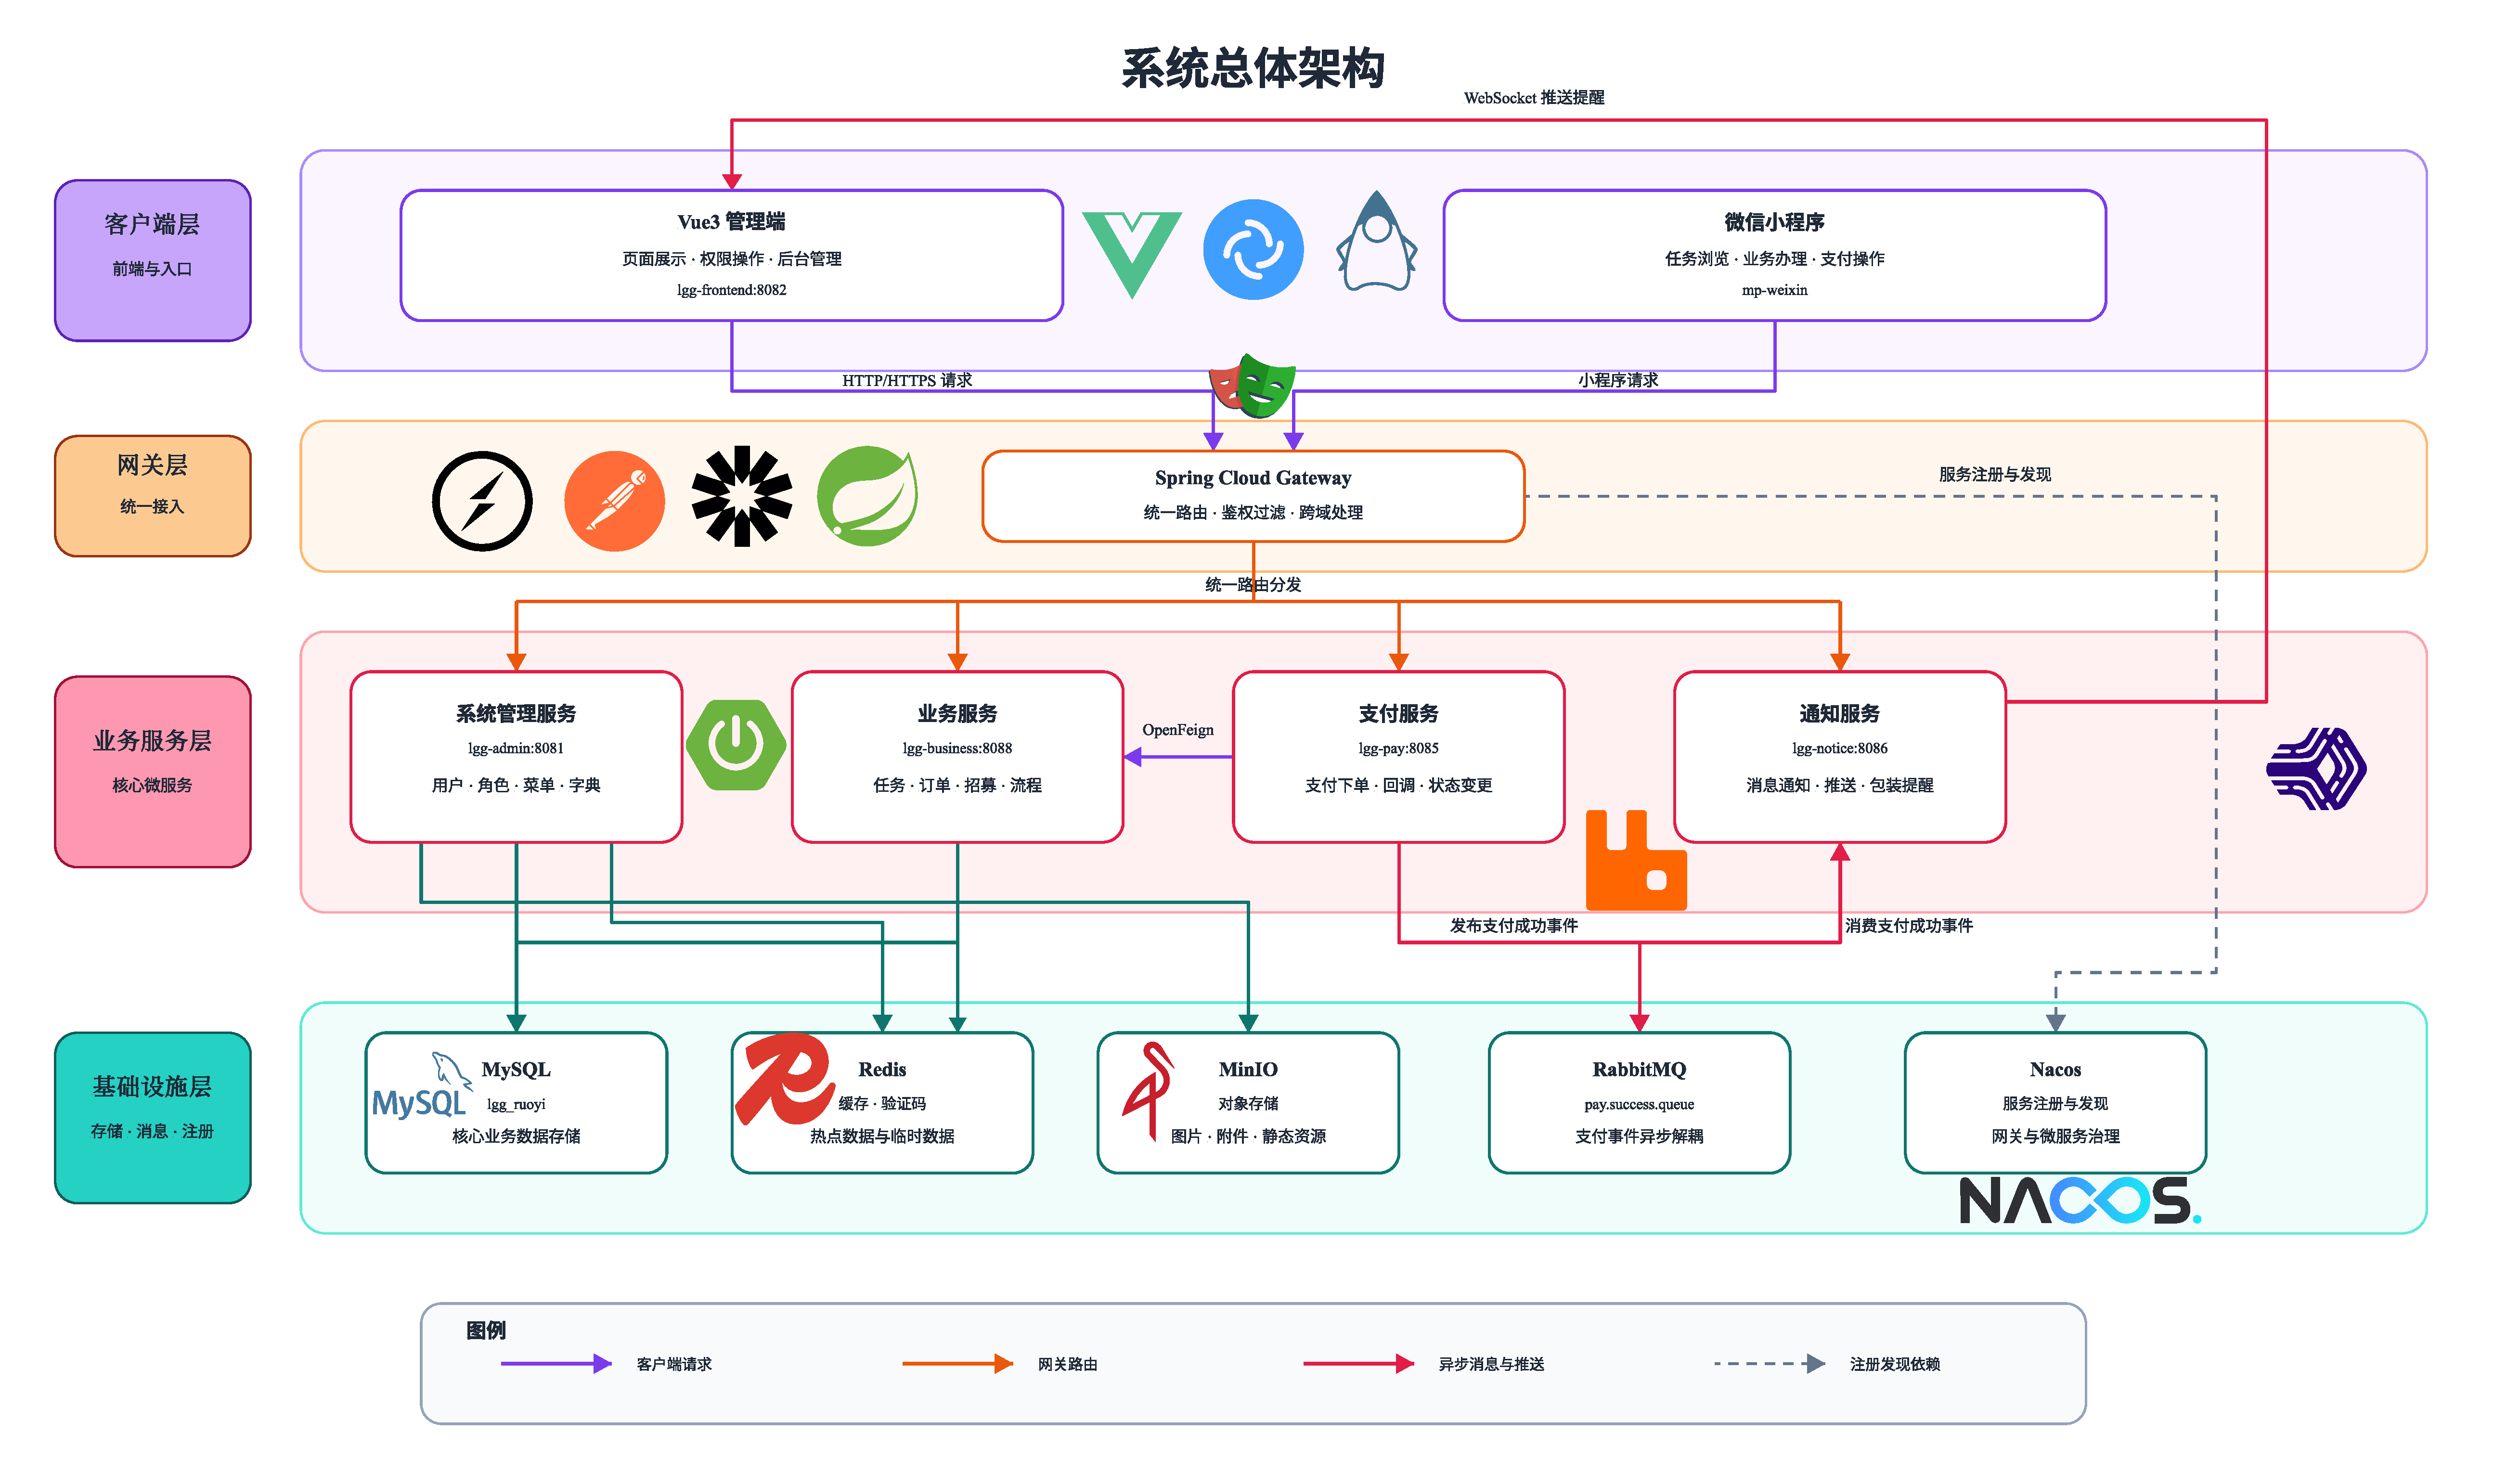
\includegraphics[width=0.9\textwidth]{figures-pdf/系统总体架构图.pdf}
  \caption{系统架构图}
  \label{fig:U01}
\end{figure}

如图 \ref{fig:U01} 所示，所有的外部请求首先流经统一 API 网关 lgg-gateway。网关通过预定义的路径断言规则执行动态路由匹配。例如，带有 /business 前缀的请求被路由至核心业务服务，带有 /pay 的请求路由至模拟支付服务。网关不仅通过全局过滤器统一解决了浏览器的 CORS 跨域问题，还自动利用 Nacos 的服务发现能力将逻辑服务名转换为物理 IP 并进行负载均衡转发。

当请求到达目标微服务后，其控制器层将调用服务层处理业务逻辑，服务层采用“先查 Redis 缓存，未命中再查 MySQL 数据库，并回写缓存”的经典数据访问模式，确保在高频读取场景下的极低延迟响应。

\section{服务模块划分}

在明确了宏观架构后，系统的分布式后端在逻辑与物理上被拆分为五个核心微服务模块。模块化设计保证了高内聚与低耦合。

\begin{figure}[htbp]
  \centering
  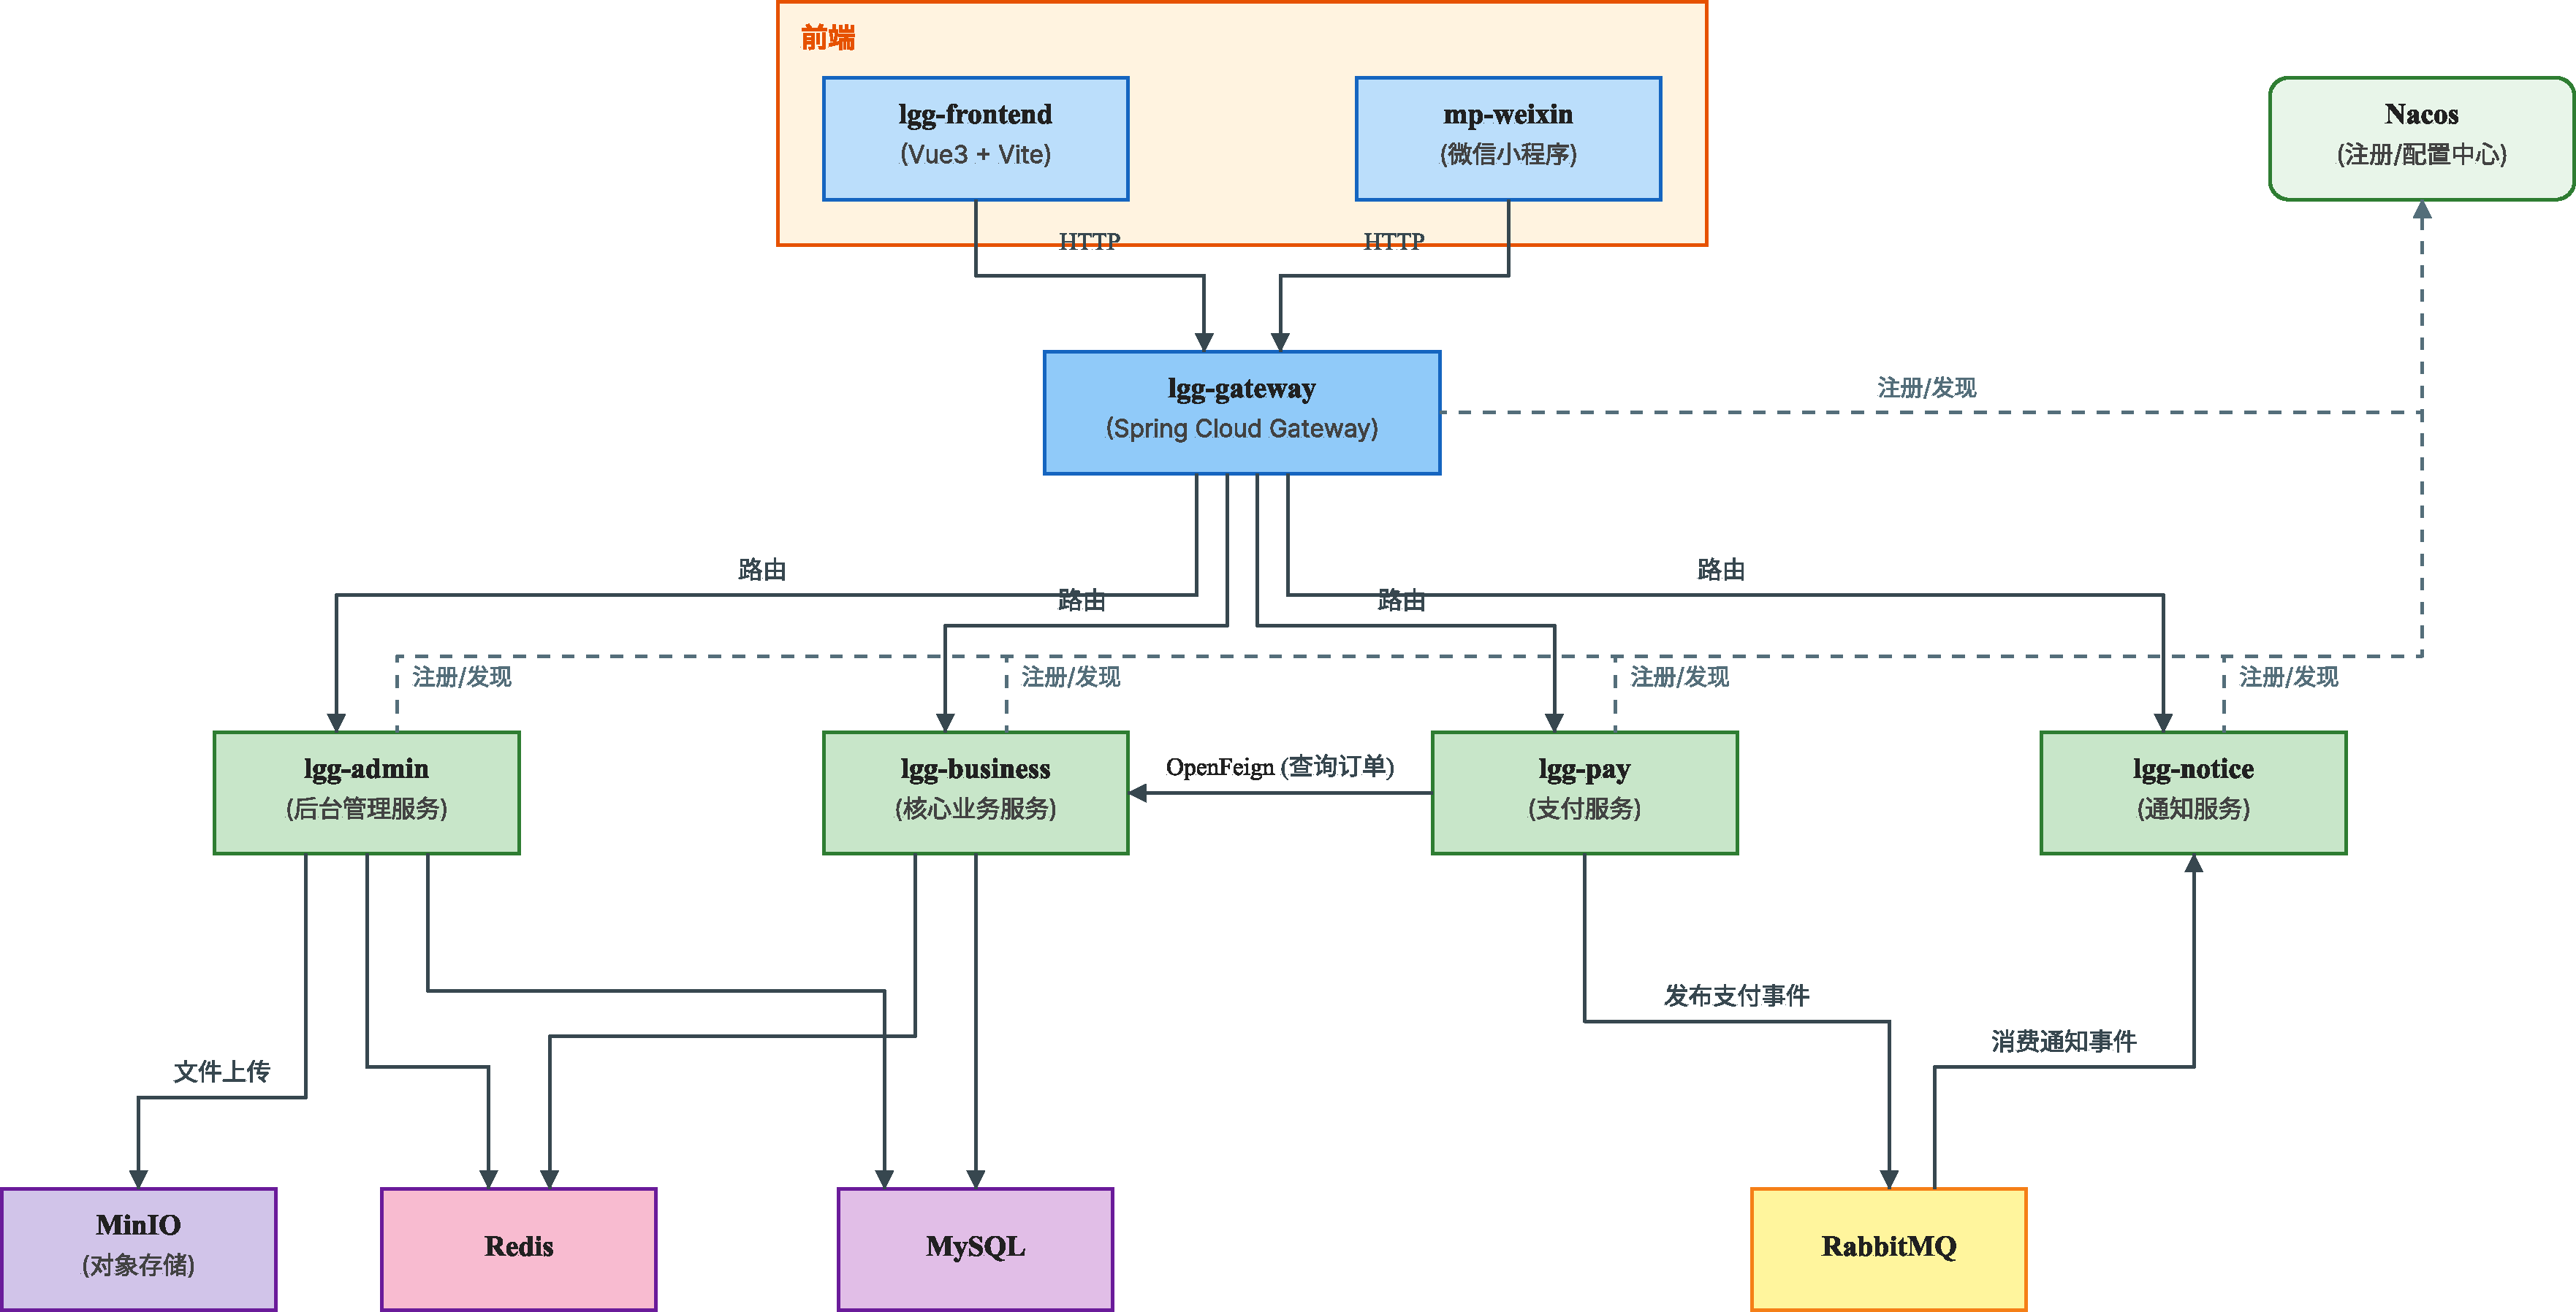
\includegraphics[width=0.9\textwidth]{figures-pdf/微服务模块依赖结构图.pdf}
  \caption{微服务模块依赖结构图}
  \label{fig:U04}
\end{figure}

由图 \ref{fig:U04} 可见，五个微服务各司其职且相互配合：
首先是 lgg-admin，它是若依管理系统的安全认证基座，负责登录鉴权与菜单下发，不与其他业务服务直接通信；其次是 lgg-business 核心业务服务，承载了最密集的分类、商品与订单持久化逻辑；接着是 lgg-pay 模拟支付服务，专门处理外部模拟回调动作，并通过 OpenFeign 同步调用业务服务；lgg-notice 则作为消息通知的末端节点，异步消费 RabbitMQ 队列；最后是 lgg-gateway 作为入口门户。各组件的具体职责如表 \ref{tab:service_components} 所示。

\begin{table}[htbp]
  \centering
  \caption{微服务核心组件与职责表}
  \label{tab:service_components}
  \begin{tabular}{lllp{0.4\textwidth}}
    \toprule
    微服务名称 & 监听端口 & 核心依赖 & 核心职责 \\
    \midrule
    lgg-admin & 8080 & MySQL, Redis & 登录鉴权、系统配置、角色权限过滤 \\
    lgg-business & 8088 & MySQL, Redis, MinIO & 分类与商品管理、购物车、订单状态更新 \\
    lgg-pay & 8085 & OpenFeign, RabbitMQ & 模拟微信扣款、触发业务回调、投递事件 \\
    lgg-notice & 8086 & RabbitMQ, WebSocket & 消费支付成功事件、推送网页端弹窗提醒 \\
    lgg-gateway & 8090 & Nacos & 全平台统一入口、跨域处理、动态路由分发 \\
    \bottomrule
  \end{tabular}
\end{table}

\section{核心业务流程与状态机设计}

在完成了静态模块的拆分后，系统设计的最后一步是对复杂的跨服务动态行为进行建模。生鲜电商的核心在于用户的下单流转以及订单状态的变化。

\begin{figure}[htbp]
  \centering
  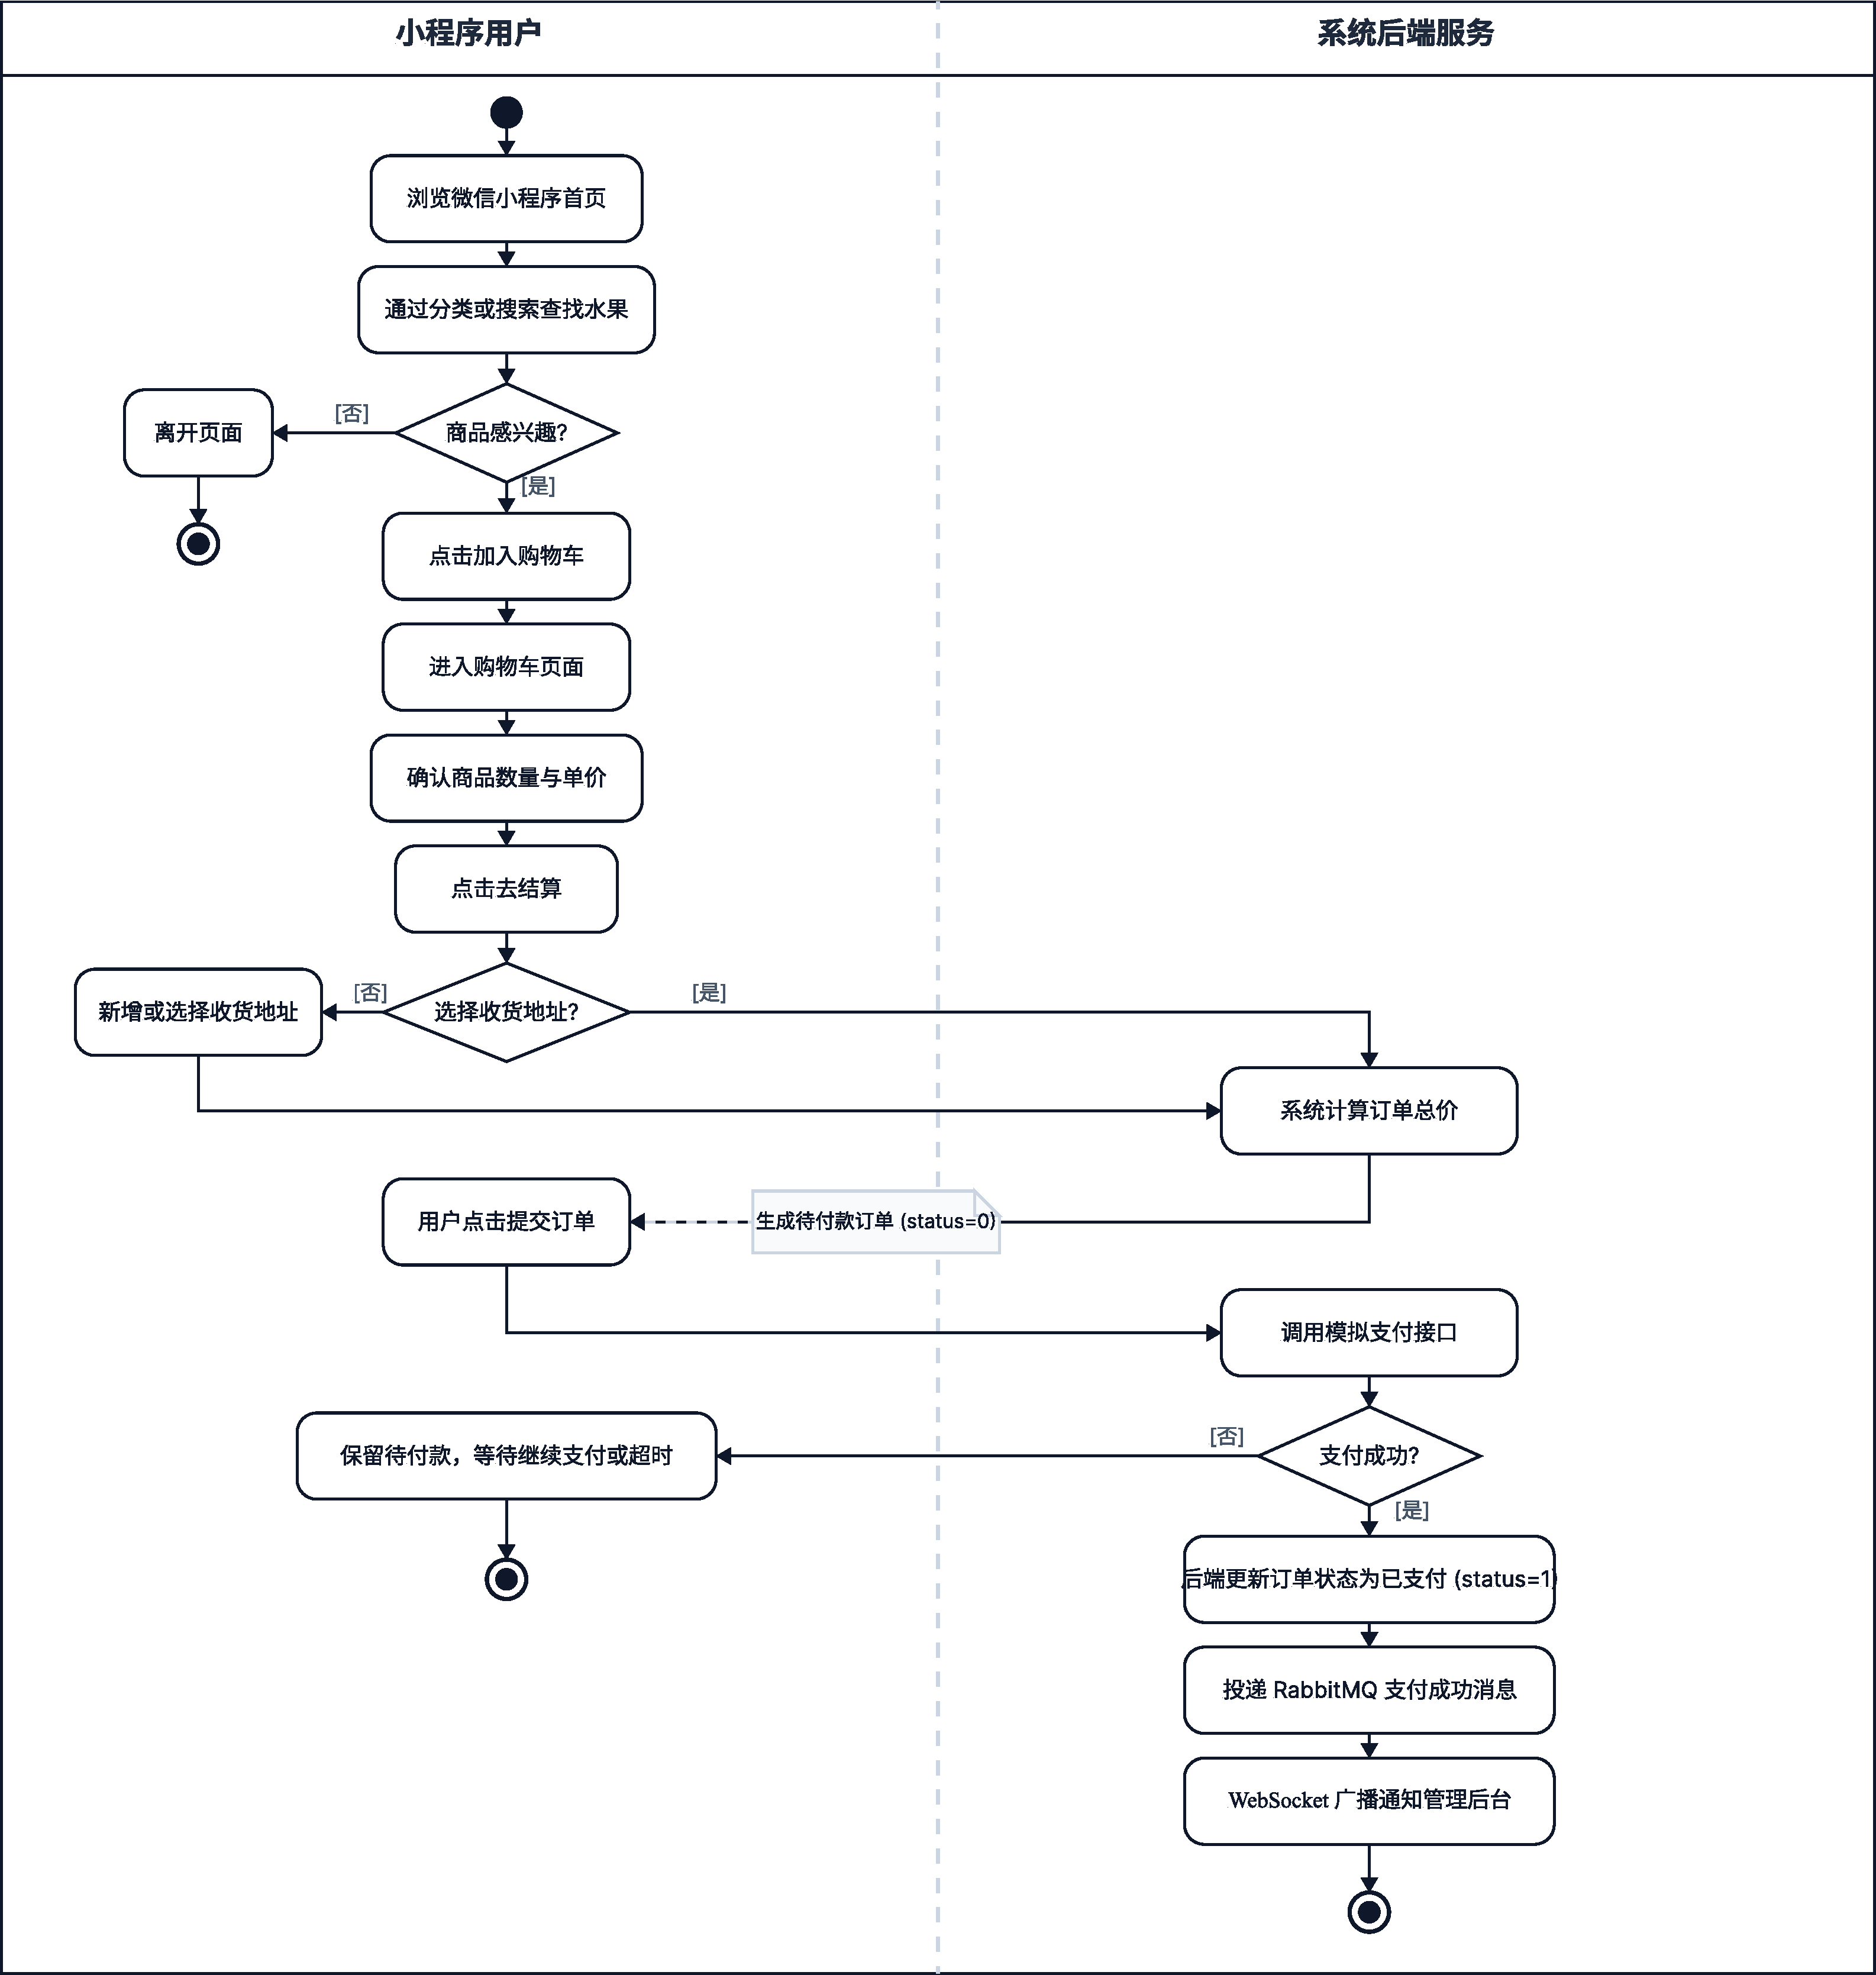
\includegraphics[width=0.9\textwidth]{figures-pdf/U06-shopping-activity.pdf}
  \caption{用户购物与支付状态流转活动图}
  \label{fig:U06}
\end{figure}

如图 \ref{fig:U06} 的全局活动图所示，从用户进入首页浏览分类开始，经过商品加入购物车、选择收货地址并确认结算，最终订单信息被持久化至数据库，初始化为待付款状态。若用户在支付页完成模拟付款操作，则正式启动后续状态闭环。

\begin{figure}[htbp]
  \centering
  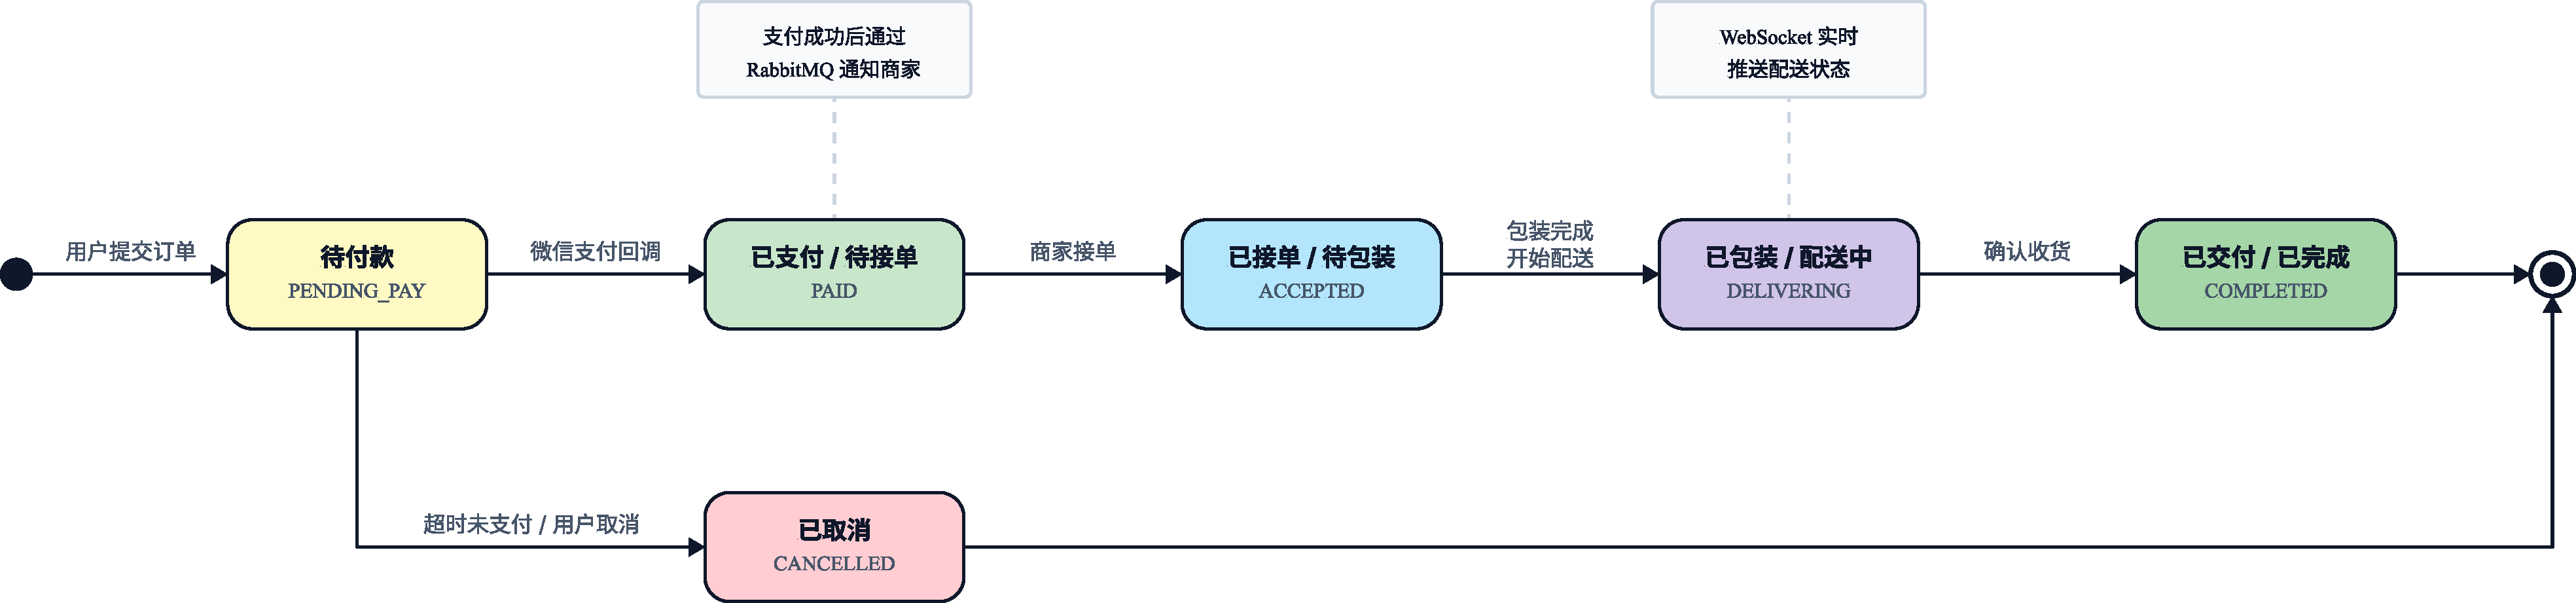
\includegraphics[width=0.9\textwidth]{figures-pdf/订单状态流转图.pdf}
  \caption{订单状态流转与消息通知流程图}
  \label{fig:U03}
\end{figure}

图 \ref{fig:U03} 详细展示了系统在订单生命周期内的状态机设计。订单必须严格遵循“待付款 -> 已支付待接单 -> 已包装待发货 -> 已完成”的单向递进规则流转。不允许任何逆向跳转或越级更新，以保障数据的审计可追溯性与业务合规性。任何试图违背该状态转移图的操作均会被后端拦截器直接驳回。

\begin{figure}[htbp]
  \centering
  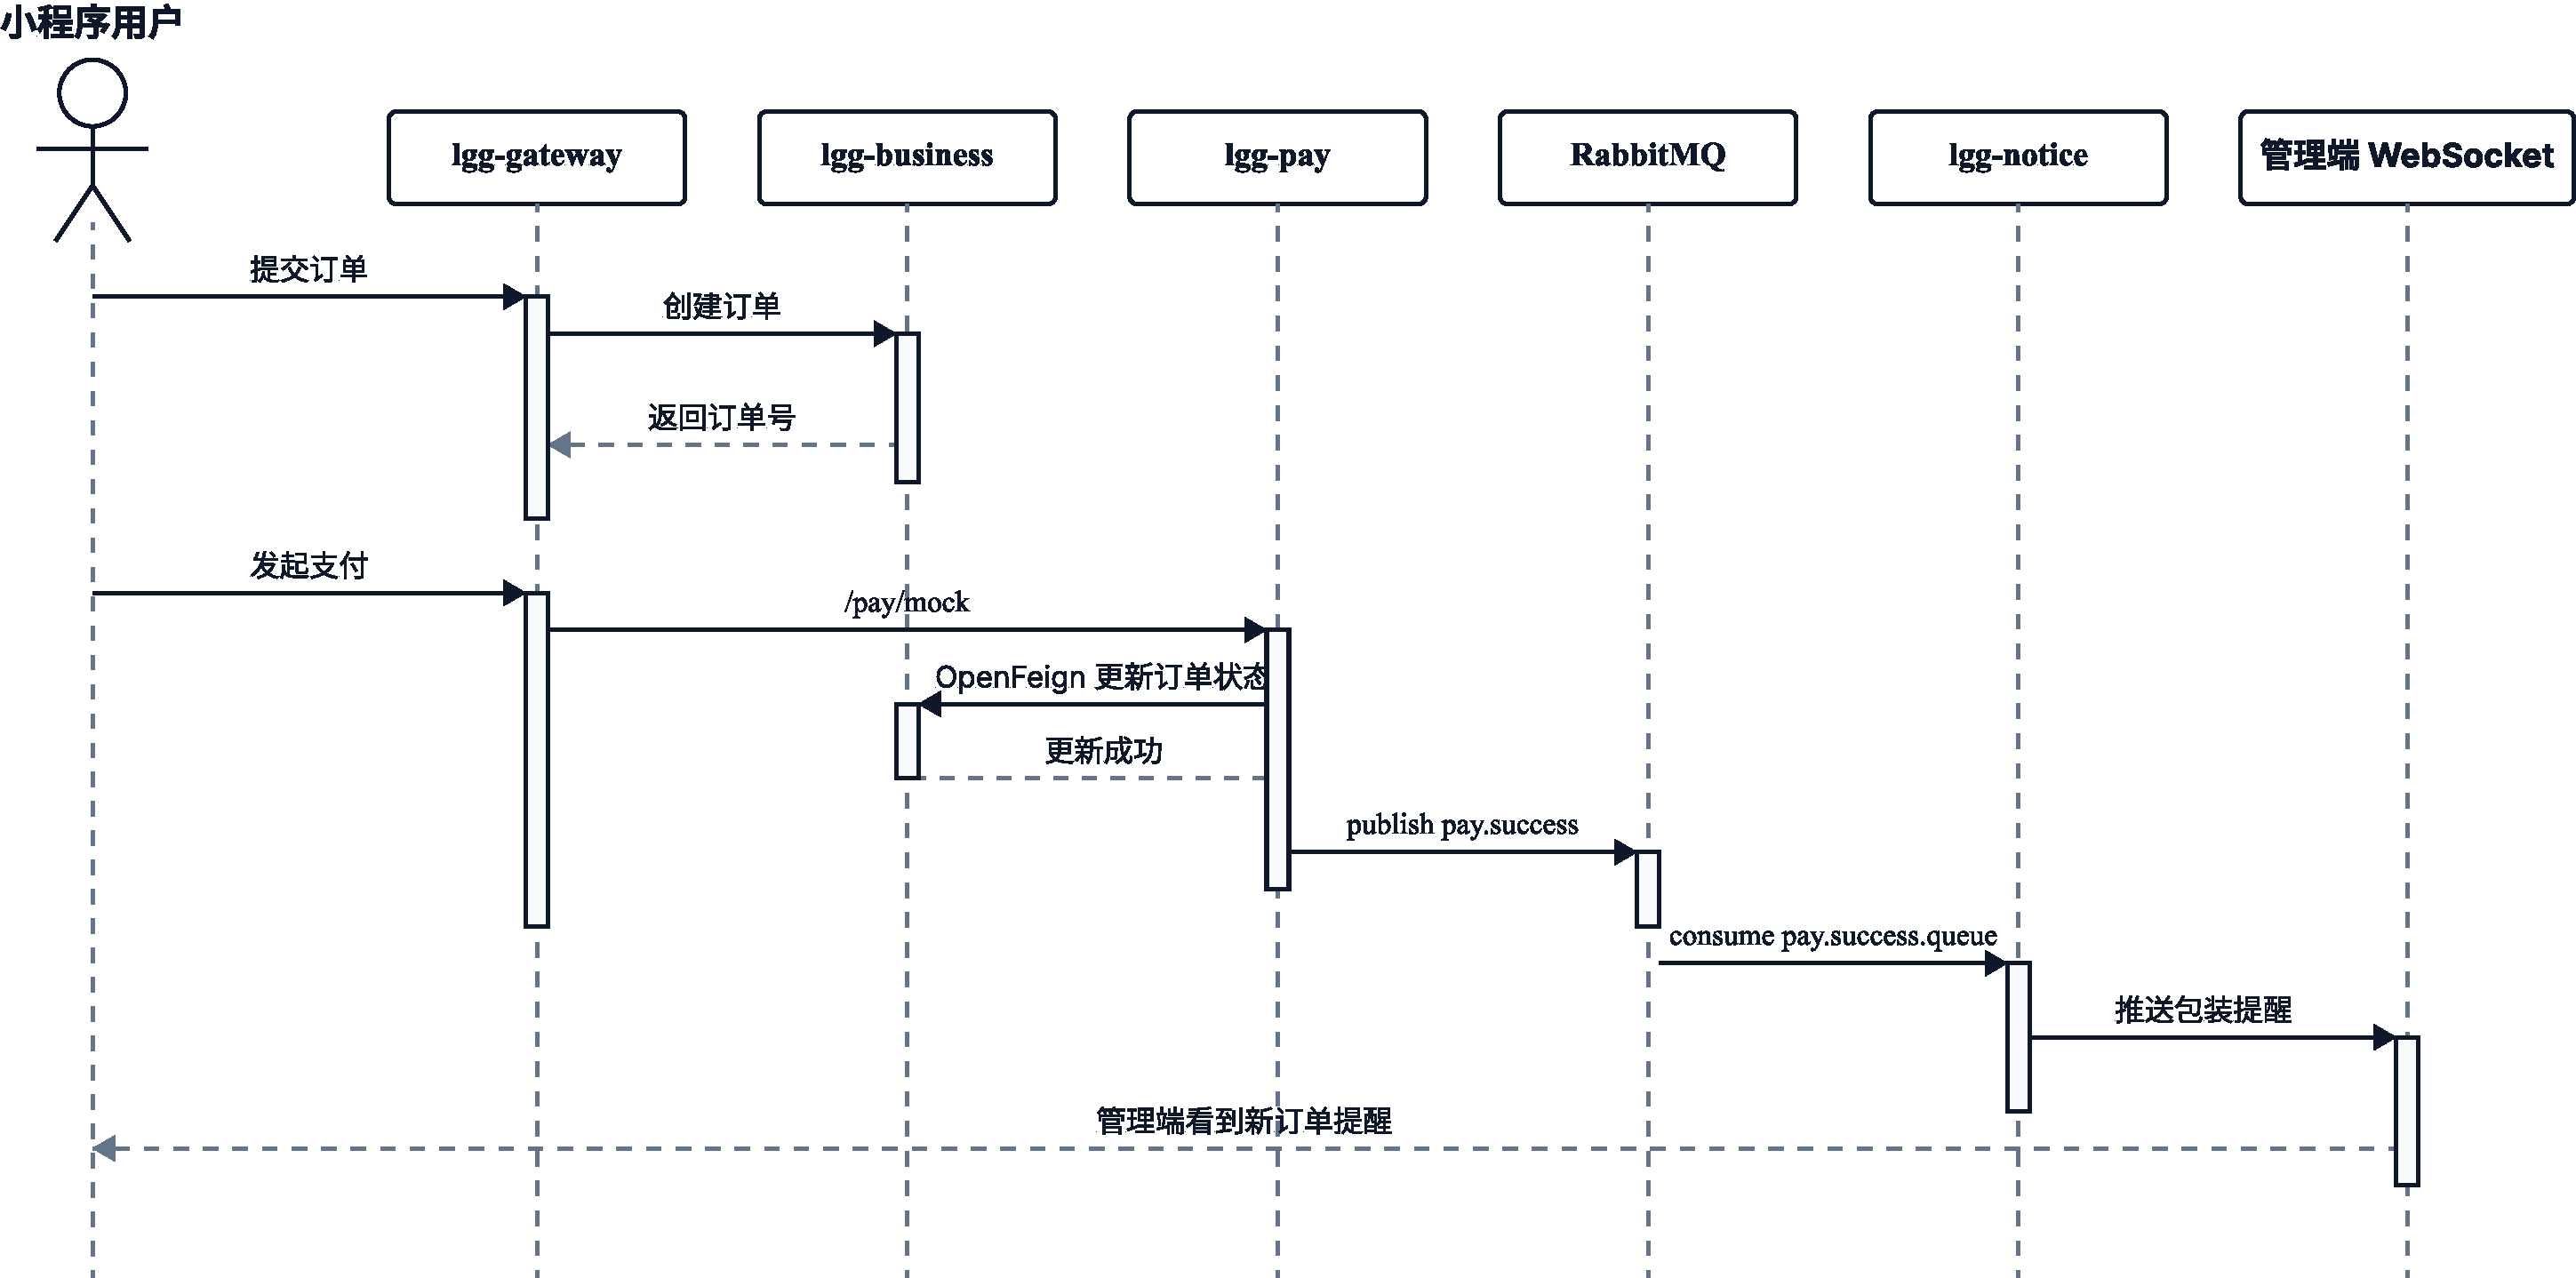
\includegraphics[width=0.9\textwidth]{figures-pdf/支付成功与包装提醒时序图.pdf}
  \caption{订单模拟支付与状态更新时序图}
  \label{fig:U02}
\end{figure}

最后，图 \ref{fig:U02} 揭示了系统内部微服务间为促成状态流转而发生的高效协作时序。当支付服务 lgg-pay 收到成功回调后，它立即利用 OpenFeign 客户端向业务服务发出同步的订单状态更新指令。在业务服务确认数据库更新成功后，支付服务紧接着向 RabbitMQ 投递异步的支付成功事件。通知服务 lgg-notice 通过订阅该队列快速捕捉事件，利用预先建立的 WebSocket 长连接将包装提醒指令推送至网页管理端。这种同步与异步结合的时序设计，既保证了数据状态的强一致性，又实现了后续非核心推送业务的弱依赖解耦。

